%!TEX root=../root.tex

%%%%%%%%%%%%%%%%%%%%%%%%%%%%%%%%%%%%%%%%%%%%%%%%%%%%%%%%%%%%%%%%%%%%%%%%%%%%%%%%
%2345678901234567890123456789012345678901234567890123456789012345678901234567890
%        1         2         3         4         5         6         7        
\section{NUMERICAL SIMULATION}
In order to verify the proposed switched \ac{lqr} for the modular model, we apply rapid prototyping in MATLAB/SIMULINK. The robot geometric configuration parameters are adapted from the \emph{Snookie} robot configuration described in~\cite{c9}, which serves as a baseline. The robot possesses four horizontal thrusters, two vertical thrusters, two horizontal fins and two vertical fins as actuators, see Fig~\ref{snookie}. The thrust force is constrained to a range of $[-35\textup{N},40\textup{N}]$ , and the deflection angle is constrained within $[-20^\circ,20^\circ]$. The desired trim paths consist of seven segments whose parameters are specified in Table~\ref{TABLE:TrimSpecifications}. The robot should track the seven trajectories in $150$ seconds. Note that the yaw rate $\dot{\phi}_{\mathcal{T}}$ can not be set to zero due to the singularity problem of (\ref{EQ:pT}). Instead, we use a very small value ($10^{-6}$) to tackle this problem. From the specifications and geometric configuration parameters, we can derive the linearized error systems for each trim trajectory segment: $A_{E,1}, \cdots, A_{E,7}$ and $B_{E,1}, \cdots, B_{E,7}$. The initial state error $\vec{x}_{E,1}$ is set to be $\vec{0}$. The drag coefficient $c_{D}$ and lift coefficient $c_{L}$ are set to be equal $0.1$ and $0.001$, respectively. 

\begin{figure}[htb]
	\begin{center}
		\includegraphics[width=.3\textwidth]{figures/Cotesys_Snookie_150dpi}
		\caption{\emph{Snookie} \ac{auv}}
		\label{snookie}
	\end{center}
\end{figure}
   
\begin{table}[htb]
\caption{Trim trajectories specifications}
\label{TABLE:TrimSpecifications}
\begin{center}
\begin{tabular}{| c | c | c | c | c |}
\hline
Segment&Time(s)&$||\vec{v}_{\mathcal{T}}||$ (m/s)&$\dot{\psi}_{\mathcal{T}}$ (rad/s)&$\gamma_{\mathcal{T}}$ (rad)\\ \hline
1&0-20&0.5&0&0\\ %\hline
2&20-30&0.5&0.0803&0 \\ %\hline
3&30-40&0.5&0.0803&0.2 \\ %\hline
4&40-50&0.5&0&0.2 \\ %\hline
5&50-60&0.5&-0.0803&0.2 \\ %\hline
6&60-70&0.5&-0.0803&0 \\ %\hline
7&70-150&0.5&0&0 \\ \hline
\end{tabular}
\end{center}
\end{table}  
 The state cost matrices for the individual trim segments are: 
\begin{align*}
	\mathcal{Q}_{1/2/4/5}&=diag([10^3, 10^3, 10^3, 300, 300, 300, 1, 1, 1, 1, 1, 1])\\
	\mathcal{Q}_{3}&=diag([10^3, 10^3, 10^3, 1, 1, 1, 1, 1, 1, 1, 1, 1])\\
	\mathcal{Q}_{6/7}&=diag([10^3, 10^3, 10^3, 10^3,  10^3, 10^3, 1, 1, 1, 1, 1, 1]),
\end{align*}
 The input weighting matrices are:
\begin{align*}
	\mathcal{R}_{2/3/4/5}&=diag([10^{-4},~\ldots~,10^{-4}, 10^{-3}, 10^{-3}, 10^{-3}, 10^{-3}])\\
	\mathcal{R}_{1/6}&=diag([10^{-4},~\ldots~,10^{-4}]) ~ \in \mathbb{R}^{12 \times 10}\\
	\mathcal{R}_{7}&=diag([10^{-5},~\ldots~,10^{-5}, 10^{-4}, 10^{-4}, 10^{-4}, 10^{-4}])
\end{align*}
Using these values, we can design an \ac{lqr} for each linearized error system and obtain state feed back gains $\mathcal{K}_{1}, \cdots, \mathcal{K}_{7}$.

In order to ensure the global stability of the formulated switched system under implementation of the \ac{lqr} with the selected weighting matrices, we check the existence of the common symmetric matrix $\mathcal{P}_{E}$ by solving the following optimization problem: 
\begin{equation}
	\min_{\mathcal{P}_{E}\in \mathbb{R}^{12 \times 12}}\mathrm{tr}(\mathcal{P}_{E}),
\end{equation} 
subject to $\bar{A}_{E,j}^{T}\mathcal{P}_{E}+\mathcal{P}_{E}\bar{A}_{E,j} \preceq I_{12 \times 12}$, $\mathcal{P}_{E} \succeq I_{12 \times 12}$, where $\bar{A}_{E,j}=A_{E,j}-\mathcal{K}_{j}$, $j=1, \cdots, 7$. Using the semidefinite programming in CVX~(\cite{c12,c13}), we could obtain the optimization result. For the current values of state cost matrices and input cost matrices, the objective function $\mathrm{tr}(\mathcal{P}_{E})$ has a feasible solution of $1891.49$, such that the corresponding positive definite symmetric matrix $\mathcal{P}_{E}$ can be used to prove the global stability of the linear switched error system. 

The reference trim trajectories and the tracked path of the underwater robot during the simulation are illustrated in Fig.~\ref{FIG:TrackingResult} and the corresponding error states $\vec{p}_{E}, \vec{\eta}_{E}, \vec{v}_{E}, \vec{w}_{E}$ are shown in Fig~\ref{FIG:ErrorStates}. If there is no actuator constraint, the robot can realize perfect tracking with the switched \ac{lqr}. For practical implementation, the control inputs are constrained by the capabilities of the actuators, as illustrated in Fig.~\ref{FIG:ControlInputs}. For tracking the first and the second trim segment along which the flight angle equals zero, the robot can nearly realize perfect tracking. When it moves downwards with flight angle $0.2$ rad, all error states rise and oscillate obviously, especially the pitch error $\vec{\theta}_{E}$. Another increase of state errors happens at the moment when the flight path angle $\gamma_{T}$ falls from $0.2$ to $0$. The changing of flight angle results in huge error and strong oscillations of the pitch error. At $70$ seconds, the yaw rate becomes zero suddenly, with a large roll velocity error $\vec{p}_{E}$ appearing consequently. Although we implement an \ac{lqr} for each trim trajectory segment, the controller can not drive the error states to zero before switching to the next trim segment. The remaining errors are the initial values for the next error dynamic system. In order to show the convergence performance of the error states under the implemented \ac{lqr}, we extend the duration of the last trim segment to $80$ seconds. From Fig.~\ref{FIG:ErrorStates}, we can see that the error states converge gradually to zero. 

\begin{figure}[htb]
\centering
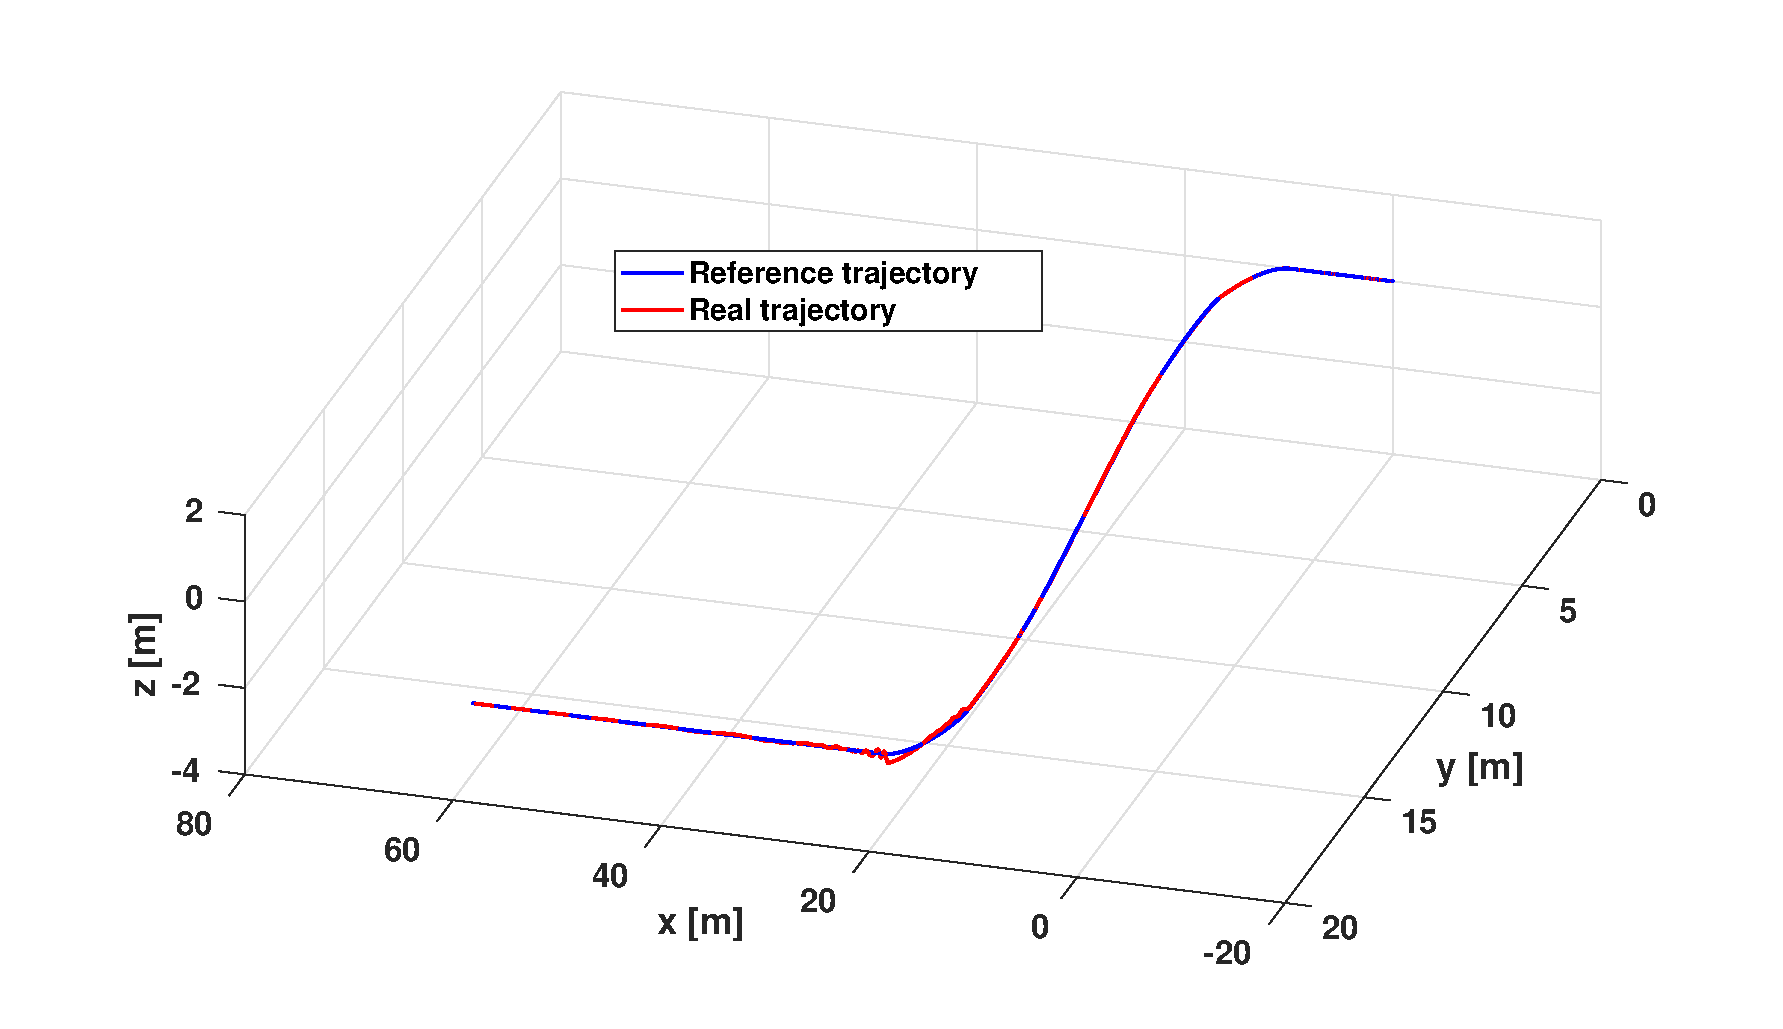
\includegraphics[width=3.5in]{TrajTracking.eps}
\caption{Tracking result}
\label{FIG:TrackingResult}
\end{figure}
\begin{figure}[htb]
\centering
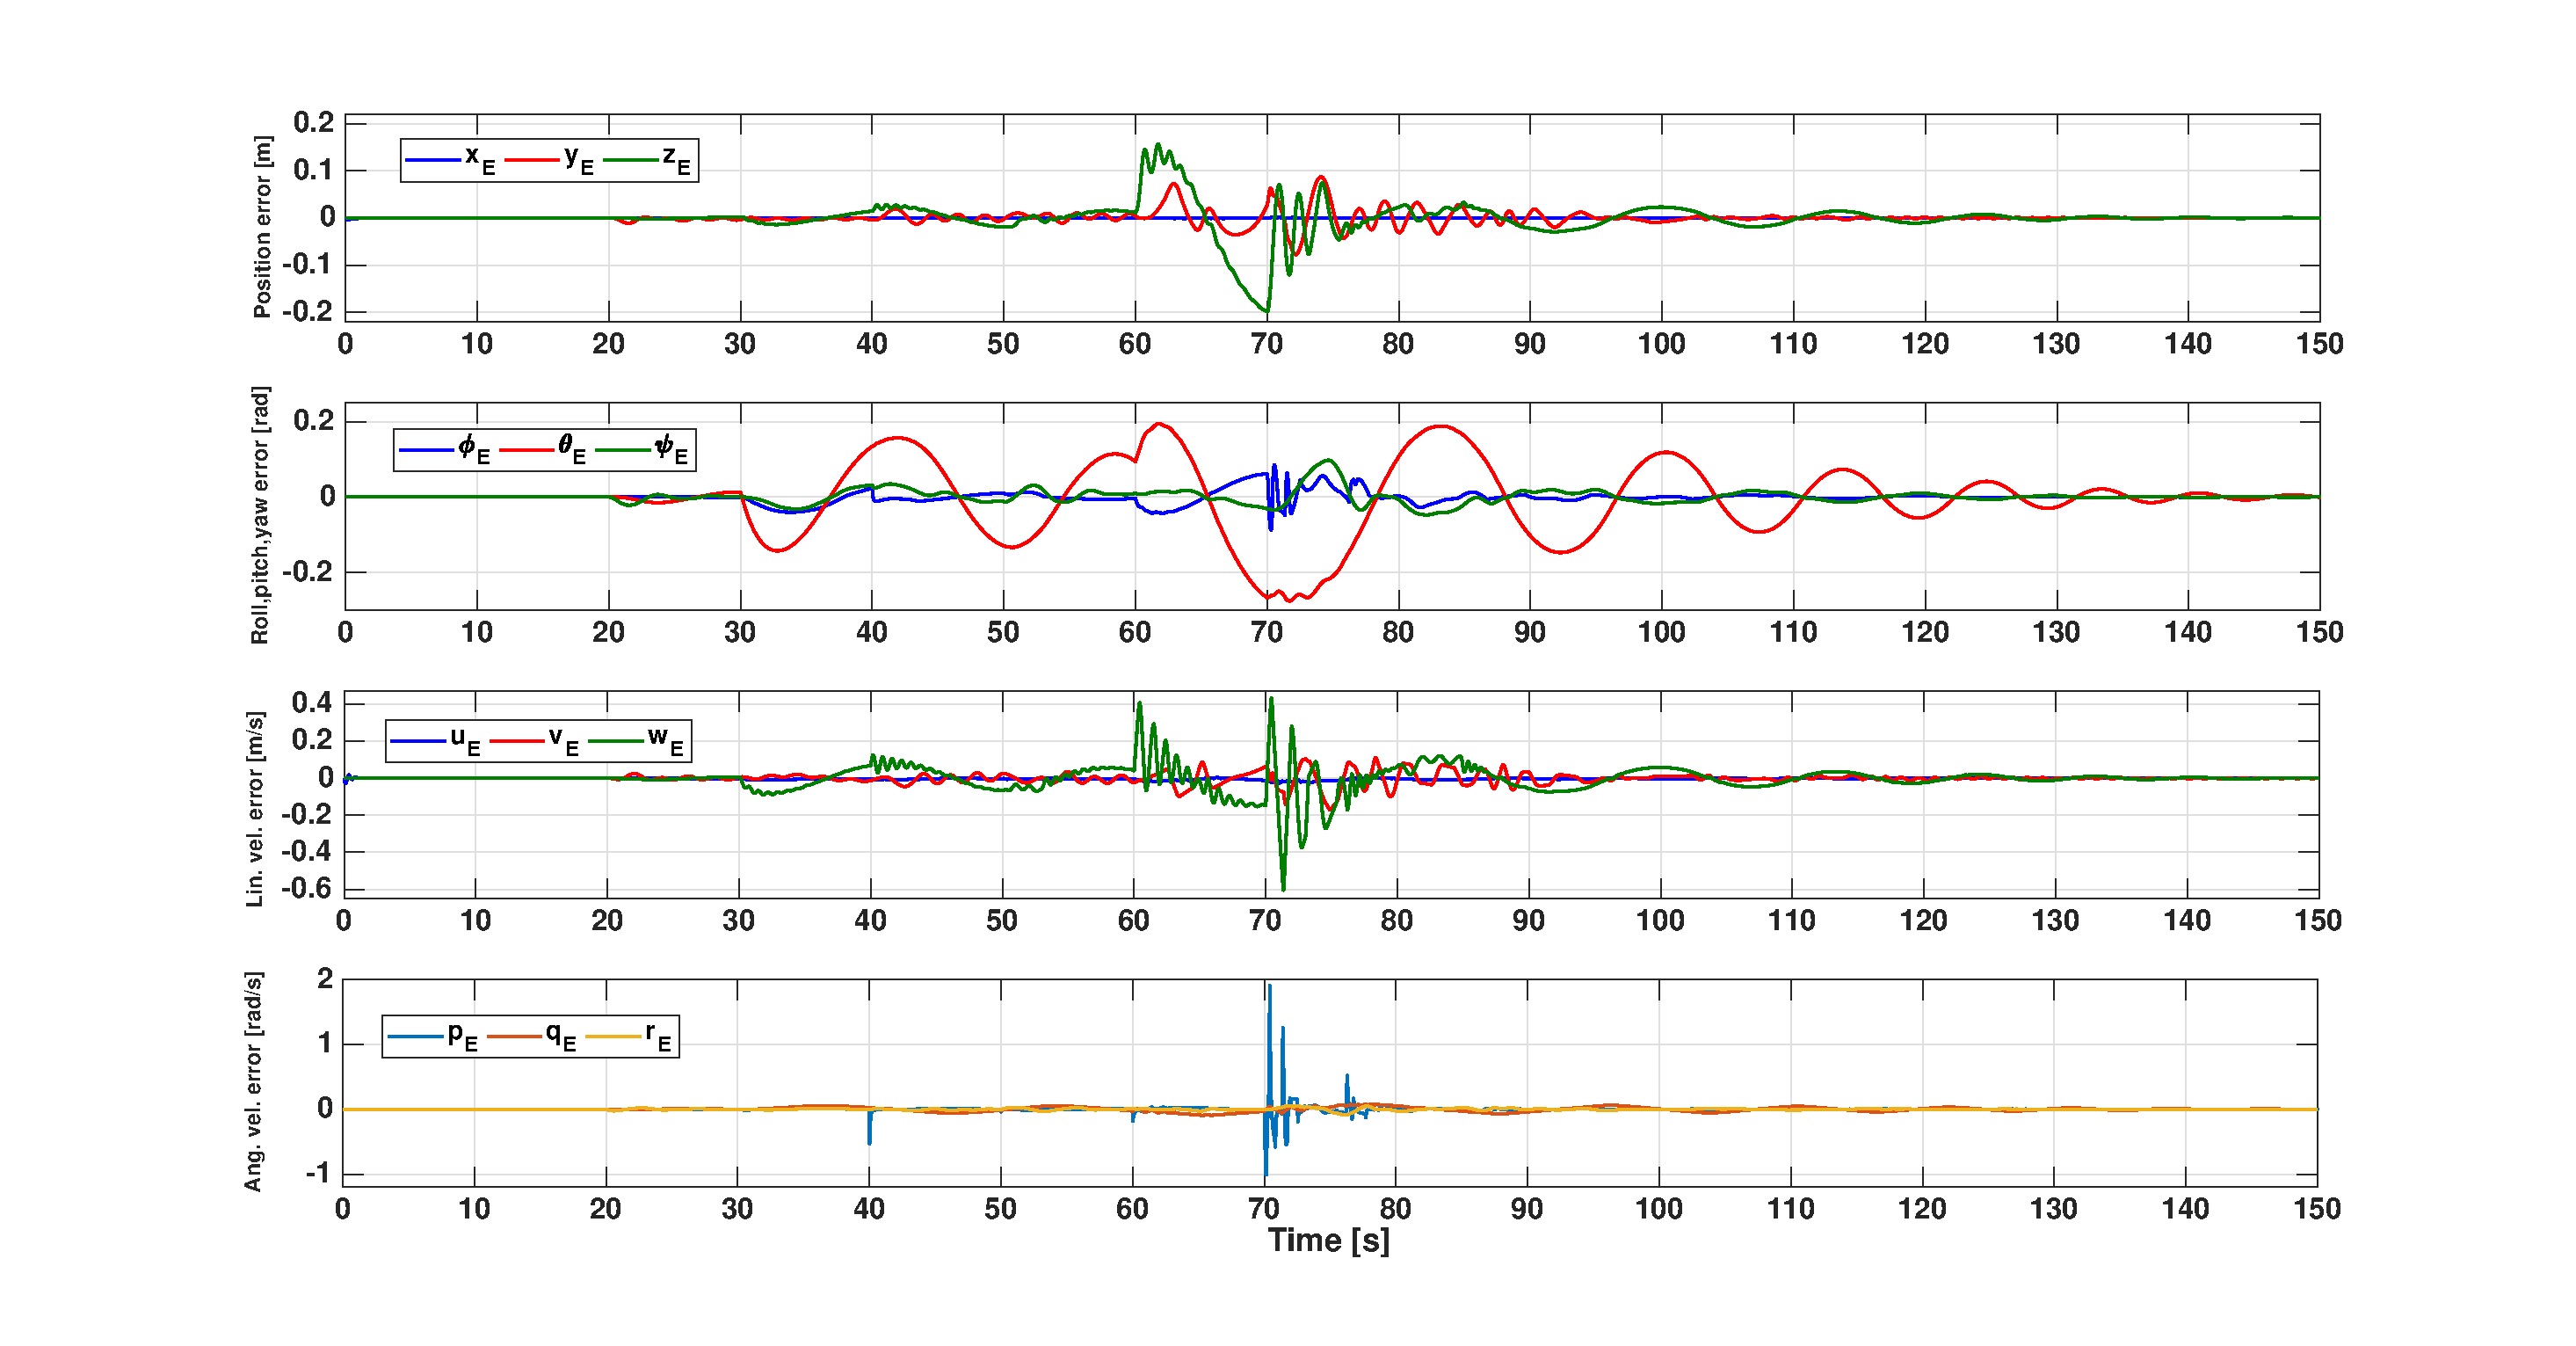
\includegraphics[width=3.5in]{StateError.eps}
\caption{Error states}
\label{FIG:ErrorStates}
\end{figure}

\begin{figure}[thpb]
\centering
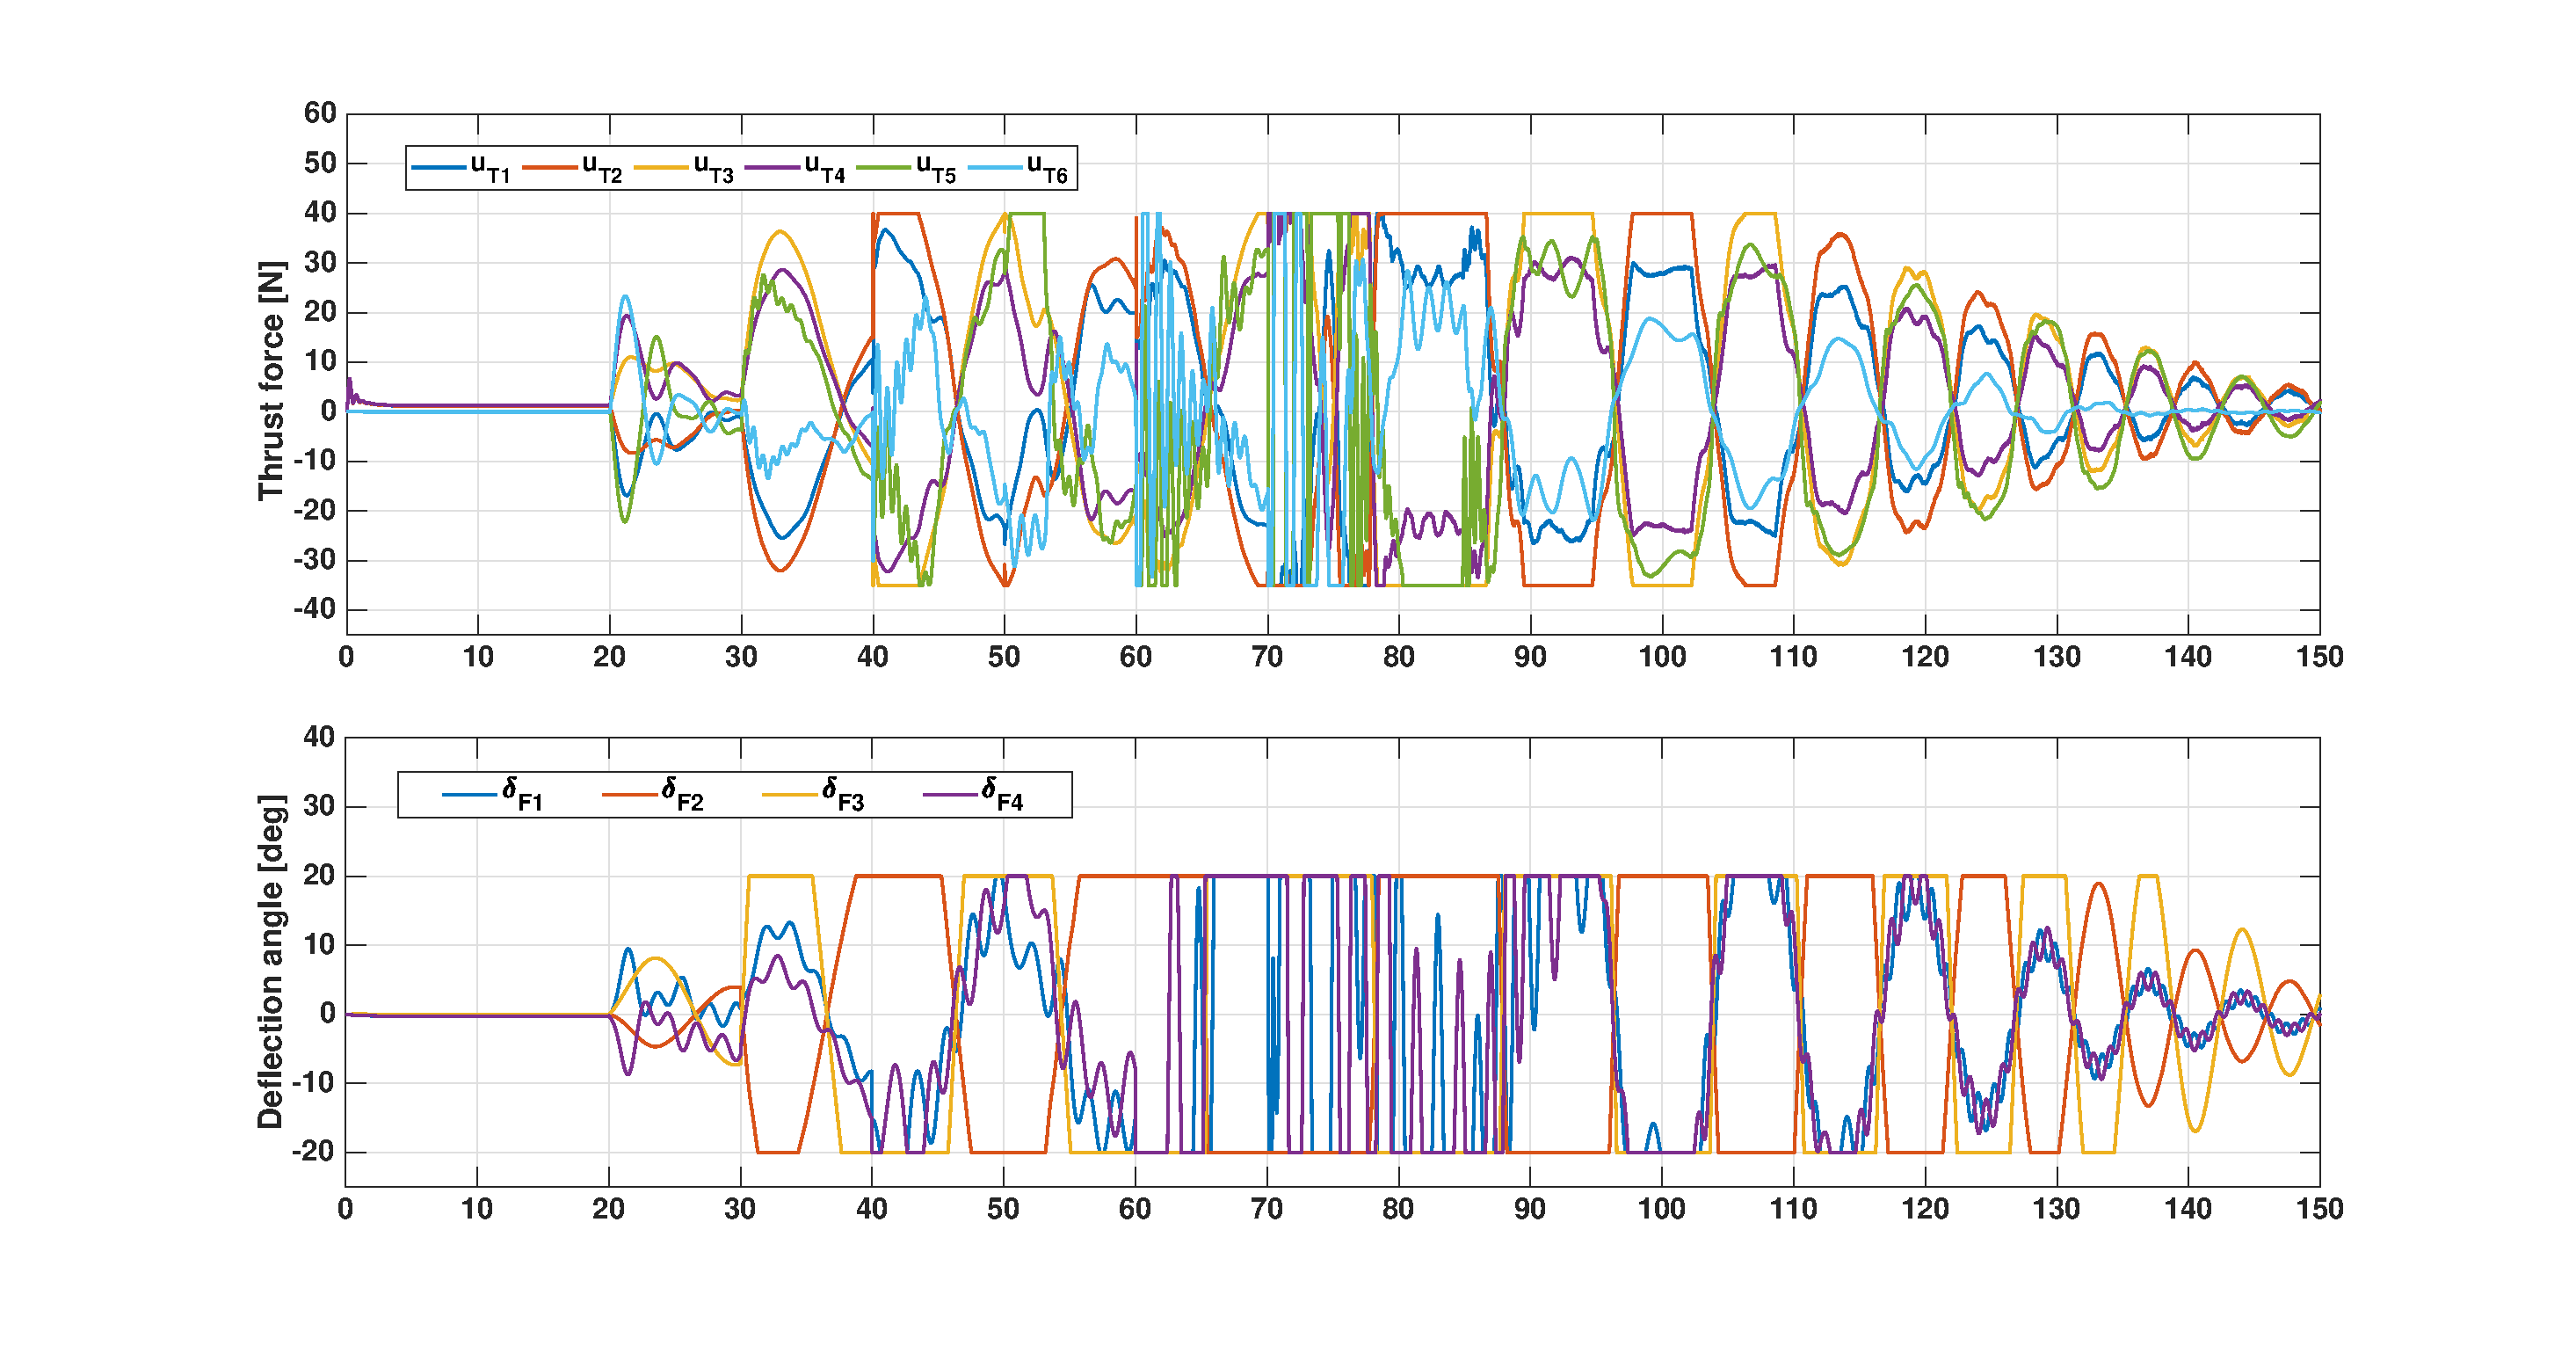
\includegraphics[width=3.5in]{InputPlot.eps}
\caption{Thrust force and deflection angle}
\label{FIG:ControlInputs}
\end{figure}

In summary, each trim path switching leads to a deviation of the real trajectory from the desired one. A switched \ac{lqr} control strategy with suitably chosen state and input weighting matrices can ensure the global stability and drive the robot to track the reference trajectory.

